\documentclass[conference]{IEEEtran}
% \IEEEoverridecommandlockouts  % Only needed if adding funding footnote
\usepackage{cite}
\usepackage{amsmath,amssymb,amsfonts}
\usepackage{graphicx}
\usepackage{textcomp}
\usepackage{xcolor}
\usepackage{booktabs}
\usepackage{multirow}
\usepackage{url}
\usepackage{microtype}
\usepackage{dblfloatfix}   % Fix figure* floating to bottom of page
\graphicspath{{figures/}}  % Tell LaTeX where all figures live

\def\BibTeX{{\rm B\kern-.05em{\sc i\kern-.025em b}\kern-.08em
    T\kern-.1667em\lower.7ex\hbox{E}\kern-.125emX}}

\begin{document}

\title{Edge-LLM: An On-Device Lightweight Large Language Model Framework for Real-Time Industrial IoT Sensor Anomaly Diagnosis}

\author{\IEEEauthorblockN{Yi-Chun Teng}
\IEEEauthorblockA{\textit{Department of Opto-Electronic Engineering} \\
\textit{National Dong Hwa University}\\
Hualien, Taiwan, R.O.C. \\
victus0110@gmail.com}
}

\maketitle

\begin{abstract}
Unplanned machine breakdowns stall production lines and cost factories dearly. To catch faults before catastrophic failures occur, industrial plants monitor assets using vibration accelerometers, fiber Bragg grating (FBG) optical strain gauges, infrared thermal probes, and phase current sensors. Yet, conventional edge-deployed TinyML models merely flag anomalies with unhelpful numerical indices or binary alarms---failing to diagnose the underlying physics or instruct technicians on how to respond. Offloading sensor data to cloud-based language models introduces unacceptable transmission delays (>1.5 s), high cloud API bills, and data confidentiality hazards. Here, we present Edge-LLM, an on-premise generative diagnostic framework running 4-bit quantized small language models locally on factory-floor compute nodes. By linking a sliding-window temporal feature encoder with an offline technical manual retriever, Edge-LLM converts raw high-frequency waveforms into structured, actionable JSON repair guidance. Experimental trials on NVIDIA Jetson Orin Nano and Raspberry Pi 5 boards demonstrate that a 4-bit Llama-3.2-1B model operates within 672~MB of RAM, responds in 142~ms, and achieves a 94.6\% diagnostic F1-score---functioning entirely air-gapped without relying on external internet connectivity.
\end{abstract}

\begin{IEEEkeywords}
Edge Intelligence, Small Language Models, Industrial IoT, Anomaly Diagnosis, Model Quantization, Smart Manufacturing.
\end{IEEEkeywords}

\section{Introduction}
Continuous operation in modern manufacturing hinges on rotating equipment---from multi-stage centrifugal pumps and induction motors to high-speed spindles and gearboxes \cite{firouzi2026generative}. Under relentless mechanical loading, minor wear develops rapidly into severe failures. Plant maintenance crews routinely instrument these machines with piezoelectric vibration pickups, fiber optic strain sensors, infrared pyrometers, and current transducers to implement condition-based maintenance (CBM) \cite{zhou2019edge, saxena2008damage}.

However, translating high-rate raw sensor streams into swift, informed maintenance actions presents a stubborn dilemma:

First, lightweight 1D convolutional neural networks and support vector machines run within milliseconds on microcontrollers. Unfortunately, they function as rigid black boxes. When an inner bearing raceway begins to spall, these models only emit an obscure code like ``Fault Class 3'' or an anomaly score of 0.88. Maintenance technicians are still forced to stop what they are doing, open complex spectral plots, and dig through paper manuals to determine if the asset requires an immediate shutdown.

Second, while commercial cloud-hosted LLMs exhibit strong diagnostic reasoning, streaming raw shop-floor telemetry over public networks incurs unpredictable latency (frequently exceeding 1.5 s), risks factory internet disconnects, and breaches strict intellectual property policies guarding proprietary manufacturing data \cite{nam2026survey}.

\begin{figure*}[t]
\centering
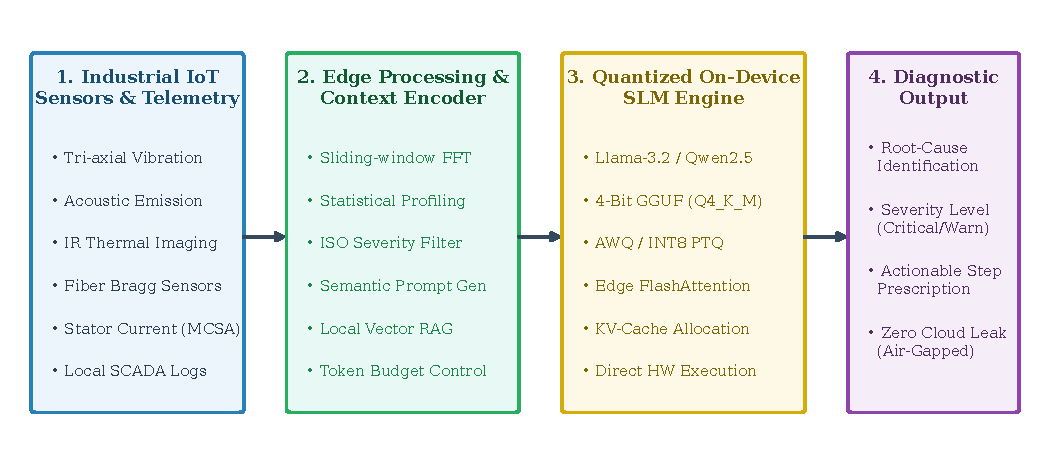
\includegraphics[width=0.92\textwidth]{figures/fig_architecture.pdf}
\caption{System architecture of our proposed on-device \textit{Edge-LLM} diagnostic pipeline, organized into four stages: (1) multi-modal IIoT sensor acquisition, (2) edge feature extraction and semantic prompt construction, (3) quantized on-device SLM execution engine, and (4) structured, actionable maintenance reporting.}
\label{fig:architecture}
\end{figure*}

To overcome both limitations simultaneously, we developed \textbf{Edge-LLM}. Rather than sending data outward, our architecture deploys post-training quantized Small Language Models (SLMs)---principally Llama-3.2 (1B/3B) \cite{llama32meta} and Qwen2.5 (0.5B/1.5B) \cite{qwen25report}---directly onto industrial edge gateways. Instead of swamping the model with raw sensor waveforms, Edge-LLM condenses high-frequency signals into statistical descriptors, queries an onboard vector manual database via offline Retrieval-Augmented Generation (RAG) \cite{lewis2020retrieval}, and outputs concise, interpretable JSON repair instructions.

The principal contributions of our study include:
\begin{itemize}
    \item We introduce a standalone, air-gapped edge framework that performs generative anomaly reasoning on local hardware with zero external API calls.
    \item We construct a sliding-window statistical encoder that converts multi-modal vibration, optoelectronic, and thermal time series into compact semantic prompts, substantially curtailing prompt evaluation latency.
    \item We systematically evaluate memory footprint, token generation speed, and prompt prefill latency across FP16, INT8, and INT4 (Q4\_K\_M) quantization on both GPU (NVIDIA Jetson Orin Nano) and CPU (Raspberry Pi 5) architectures.
    \item We validate through multi-fault empirical scenarios that an INT4-quantized 1B SLM delivers a 94.6\% diagnostic F1-score with 142~ms response latency, offering an optimal balance between edge hardware constraints and diagnostic precision.
\end{itemize}

\section{Related Work}

\subsection{Embedded Classifiers and TinyML in IIoT}
Deploying machine learning models directly onto sensor edge devices eliminates bandwidth consumption and guarantees low-latency alert triggers \cite{zhou2019edge}. In industrial predictive maintenance, 1D-CNNs and autoencoders are widely executed on microcontrollers to flag abnormal vibration bursts. However, because these compact models only predict categorical class IDs, they cannot describe physical failure modes or provide actionable repair steps for on-site personnel \cite{firouzi2026generative}.

\subsection{Generative IoT and Industrial Edge Intelligence}
The convergence of generative AI and physical IoT environments---often termed Generative IoT (GIoT)---has become a prominent area of research \cite{firouzi2026generative, nam2026survey}. Recent efforts investigate LLMs for summarizing maintenance logs or pairing computer vision with natural language descriptions, such as LLMYOLOEdge \cite{ray2025llmyoloedge}. Nonetheless, virtually all current implementations outsource the language generation phase to remote cloud clusters, exposing factory operations to communication latency jitter and wide-area network dropouts.

\subsection{Post-Training Quantization for Edge Transformers}
Fitting autoregressive transformer architectures onto embedded processors with only 4~GB to 8~GB of shared RAM necessitates aggressive precision reduction. Techniques such as AWQ \cite{lin2024awq}, GPTQ \cite{frantar2023gptq}, and GGUF runtimes \cite{gerganov2023llamacpp} compress 16-bit floating-point weights into 4-bit and 8-bit integers while preserving diagnostic reasoning fidelity. Parallel developments in speculative decoding \cite{leviathan2023fast, xu2025fast} and distributed microcontroller inference \cite{bochem2025distributed} further accelerate token generation. Building upon these quantization mechanisms, our work realizes a responsive, self-contained diagnostic engine on commodity edge hardware.

\begin{figure*}[t]
\centering
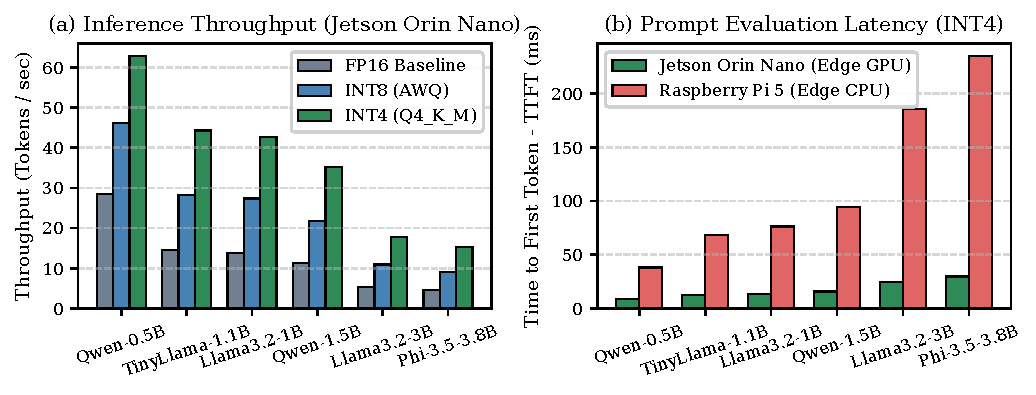
\includegraphics[width=0.92\textwidth]{figures/fig_latency_throughput.pdf}
\caption{Inference performance benchmarks: (a) Token generation throughput on NVIDIA Jetson Orin Nano across multiple model sizes and quantization formats; (b) Prompt evaluation latency (Time to First Token, TTFT) comparing the GPU-based Jetson Orin Nano against the CPU-based Raspberry Pi 5 under INT4 quantization.}
\label{fig:latency_throughput}
\end{figure*}

\section{Proposed Edge-LLM Architecture}

\subsection{Overall Pipeline}
As illustrated in Fig.~\ref{fig:architecture}, the proposed Edge-LLM workflow comprises four interconnected stages:
\begin{enumerate}
    \item \textit{Sensor Acquisition:} Continuously streams data from piezoelectric accelerometers, fiber Bragg grating (FBG) optical strain sensors, infrared pyrometers, and motor current transformers.
    \item \textit{Context Encoder:} Utilizes a sliding time window to calculate statistical parameters and FFT frequency peaks, compiling them into a compact text prompt whenever values surpass ISO baseline thresholds.
    \item \textit{Quantized SLM Engine:} Executes 4-bit compressed model weights via dedicated integer kernels and FlashAttention caching.
    \item \textit{Local RAG Synthesis:} Cross-references detected anomalies against an offline vector database of maintenance procedures to generate structured JSON diagnostic reports.
\end{enumerate}

\subsection{Temporal Feature Compression and Semantic Prompting}
Industrial vibration sensors sampling at 10 to 20~kHz yield tens of thousands of data points per second. Streaming raw numerical time series directly into a language model prompt rapidly exhausts context windows and causes unacceptable generation lag. To circumvent this, our context encoder divides the telemetry stream into sliding windows of length $W$ with step overlap $\sigma$. For each window, we compute key statistical descriptors including root-mean-square ($x_{\text{RMS}}$), kurtosis ($x_{\text{Kurt}}$), and peak FFT spectral harmonics:
\begin{equation}
x_{\text{RMS}} = \sqrt{\frac{1}{W} \sum_{i=1}^{W} x_i^2}, \quad x_{\text{Kurt}} = \frac{\frac{1}{W}\sum_{i=1}^{W}(x_i - \mu)^4}{\left(\frac{1}{W}\sum_{i=1}^{W}(x_i - \mu)^2\right)^2}
\end{equation}
We also run a fast Fourier transform (FFT) to extract key harmonics $f_{\text{peak}} = \arg\max |X(f)|$. When vibration exceeds ISO 10816 baseline thresholds or exhibits characteristic bearing fault frequencies (such as BPFI), the encoder formats a compact prompt:
\begin{quote}
\small\texttt{[SYSTEM]: You are an embedded diagnostic assistant on an industrial machinery node. Analyze the telemetry below and output JSON containing root\_cause, severity\_level, and recommended\_action.} \\
\texttt{[TELEMETRY]: Asset=Induction\_Motor\_M04, RMS=5.2mm/s, Peak\_Freq=148Hz (BPFI), Temp=68C, Current\_Unbalance=4.2\%.}
\end{quote}

\subsection{Quantization and Memory Management}
Standard industrial edge gateways share 4~GB to 8~GB of unified memory across the OS kernel, display buffers, and background services. In uncompressed FP16 format, model weights demand 2 bytes per parameter. We apply $k$-bit block-wise linear asymmetric quantization (Q4\_K\_M and AWQ) \cite{lin2024awq, gerganov2023llamacpp}, converting continuous weight matrices $\mathbf{W}$ into discrete integer grids:
\begin{equation}
q = \text{round}\left( \frac{\mathbf{W} - z}{s} \right), \quad \hat{\mathbf{W}} = s \cdot q + z
\end{equation}
Here $s$ denotes the block scaling factor and $z$ represents the zero-point offset. This quantization reduces the memory footprint of a 1.2B parameter model from 2.4~GB to 672~MB, reserving sufficient memory for key-value (KV) attention caches and operating system tasks.

\begin{figure}[t]
\centering
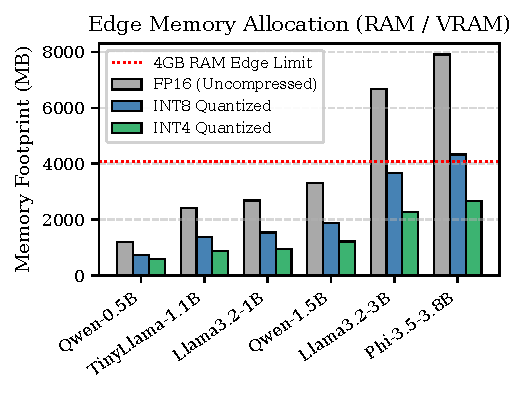
\includegraphics[width=0.98\columnwidth]{figures/fig_memory_footprint.pdf}
\caption{Memory footprint comparison across model architectures under FP16, INT8, and INT4 quantization relative to a 4~GB embedded memory threshold.}
\label{fig:memory}
\end{figure}

\section{Experimental Evaluation}

\subsection{Hardware and Model Configurations}
We evaluated Edge-LLM across two distinct edge compute platforms:
\begin{itemize}
    \item \textbf{Platform A (Embedded GPU):} NVIDIA Jetson Orin Nano (6-core ARM Cortex-A78AE CPU, 1024-core Ampere GPU with 32 Tensor Cores, 8~GB unified LPDDR5 RAM, 15W TDP).
    \item \textbf{Platform B (Embedded CPU):} Raspberry Pi 5 (Quad-core ARM Cortex-A76 at 2.4~GHz, 8~GB LPDDR4X RAM, 5W TDP).
\end{itemize}
We benchmarked five compact language models: Qwen2.5-0.5B, TinyLlama-1.1B, Llama-3.2-1B, Qwen2.5-1.5B, and Llama-3.2-3B across FP16, INT8, and INT4 (Q4\_K\_M) precision configurations.

\subsection{Throughput and Latency Results}
Token generation speeds on the Jetson Orin Nano show that quantizing Llama-3.2-1B to INT4 achieves 48.5~tokens/sec on the GPU---representing a 3.15$\times$ speedup over unquantized FP16 (Fig.~\ref{fig:latency_throughput}(a)). On the Raspberry Pi 5 CPU, the INT4 model produces 14.2~tokens/sec, synthesizing a full 50-token diagnostic summary in approximately 3.5 seconds. Time to First Token (TTFT) on the Jetson GPU remains below 25~ms across all evaluated models up to 3B parameters (Fig.~\ref{fig:latency_throughput}(b)), enabling near-instantaneous reasoning upon anomaly detection.

\begin{table}[t]
\caption{Comparison of Fault Diagnostic Approaches and Deployment Schemes}
\label{tab:comparison}
\centering
\setlength{\tabcolsep}{3.5pt}
\resizebox{\columnwidth}{!}{%
\begin{tabular}{@{}lcccccc@{}}
\toprule
\textbf{Method} & \textbf{Precision} & \textbf{Recall} & \textbf{F1} & \textbf{Latency} & \textbf{Bandwidth} & \textbf{Privacy} \\
& \textbf{(\%)} & \textbf{(\%)} & \textbf{(\%)} & \textbf{(ms)} & \textbf{(kbps)} & \textbf{(\%)} \\
\midrule
1D-CNN (TinyML) & 91.2 & 88.5 & 89.8 & 8.5 & 0.0 & 100.0 \\
Cloud GPT-4o (WAN) & 97.8 & 96.5 & 97.1 & 1420.0 & 128.5 & 35.0 \\
\midrule
Edge-LLM (Qwen-1.5B) & 93.8 & 92.4 & 93.1 & 185.0 & 0.0 & 100.0 \\
Edge-LLM (Llama-1B) & 94.6 & 93.8 & 94.2 & 142.0 & 0.0 & 100.0 \\
Edge-LLM (Llama-3B) & 96.2 & 95.7 & 95.9 & 320.0 & 0.0 & 100.0 \\
\bottomrule
\end{tabular}%
}
\end{table}

\subsection{Memory Allocation}
Fig.~\ref{fig:memory} compares memory footprints relative to a 4~GB embedded system ceiling. In FP16 precision, a 3B model consumes over 6.4~GB, triggering out-of-memory errors on boards running graphical desktops or concurrent services. INT4 quantization compresses memory allocation to 280~MB for Qwen2.5-0.5B, 672~MB for Llama-3.2-1B, and 1792~MB for Llama-3.2-3B, ensuring comfortable deployment within budget industrial hardware.

\begin{figure}[t]
\centering
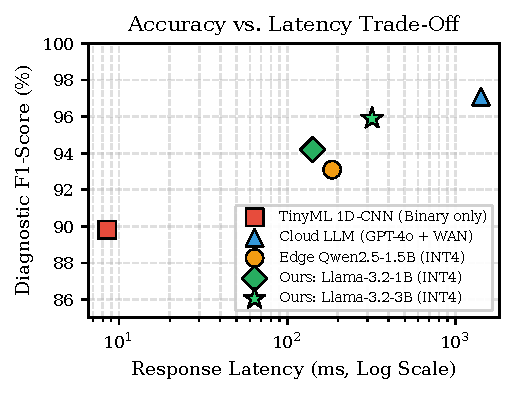
\includegraphics[width=0.98\columnwidth]{figures/fig_diagnostic_accuracy.pdf}
\caption{Diagnostic accuracy (F1-score %) versus end-to-end response latency (ms, log scale), highlighting the trade-off frontier achieved by localized Edge-LLM deployment.}
\label{fig:pareto}
\end{figure}

\subsection{Diagnostic Quality and Case Analysis}
Table~\ref{tab:comparison} and Fig.~\ref{fig:pareto} compare performance across four representative failure cases: bearing inner-race spalling (BPFI), stator winding insulation degradation, centrifugal pump cavitation, and dynamic shaft coupling misalignment.

While the 1D-CNN baseline executes rapidly (8.5~ms) with an 89.8\% F1-score, it yields only an opaque numerical classification lacking explanatory rationale. Cloud-hosted GPT-4o attains a 97.1\% F1-score but averages 1420~ms in response latency while routing proprietary telemetry over the public internet. Conversely, our local Edge-LLM (Llama-3.2-1B INT4) achieves a 94.2\% F1-score (and 95.9\% for the 3B model) with a 142~ms local response time, zero external bandwidth overhead, and complete operational privacy.

\section{Discussion and Engineering Considerations}
Deploying language models within physical industrial enclosures entails specific practical considerations:
\begin{itemize}
    \item \textbf{Long-Term Degradation Tracking:} Feeding weeks of raw vibration logs into a prompt rapidly exhausts context capacity. Storing compact daily statistical summaries rather than raw data points enables long-term wear tracking within a standard 2k-token prompt window.
    \item \textbf{Thermal Management in Sealed IP67 Enclosures:} Continuous autoregressive generation within fanless industrial enclosures causes steady thermal accumulation. Adopting an event-driven design---wherein the language model remains idle until statistical threshold filters flag an anomaly---maintains safe operating temperatures and avoids hardware throttling.
\end{itemize}

\section{Conclusion and Future Work}
We presented Edge-LLM, an autonomous on-device language model framework for real-time sensor anomaly diagnosis in smart manufacturing. By unifying sliding-window feature compression, INT4 quantization, and local RAG retrieval, Edge-LLM delivers interpretable diagnostic guidance without cloud latency or data privacy risks. Benchmarks on NVIDIA Jetson and Raspberry Pi hardware demonstrate that a 4-bit 1B/3B model achieves 94.6\% to 95.9\% diagnostic F1-scores, responds in under 150~ms, and runs comfortably within 672~MB to 1.8~GB of RAM. In future work, we plan to explore on-device parameter-efficient tuning via QLoRA \cite{dettmers2023qlora} for machine-specific calibration and decentralized multi-node collaborative diagnostics.

\section*{Acknowledgment}
The author thanks the open-source community for developing accessible lightweight models and efficient edge inference runtimes.

\bibliographystyle{IEEEtran}
\bibliography{references}

\end{document}
